\subsection{Constituent Counting Rule}
The constituent counting rule (CCR) predicts the energy dependence of the differential cross-section at fixed center-of-mass angles for an exclusive two-body reactions. It validity is at high beam energies and large momentum transfer and the framework is similar to that of the handbag approach, in which the theory relies on the factorization of the exclusive process into a hard scattering amplitude and a soft quark amplitude inside the hadron. The prediction of CCR is:
\begin{equation}
\frac{d\sigma}{dt} \sim s^{2-n}f(\theta_{c.m.}) \label{CCR}
\end{equation}
where $s$ and $t$ are the Mandelstam variables, $n$ is the total number of interacting elementary fields in the initial and final state of the reaction and $f(\theta_{c.m.})$ depends on the dynamics of the process. Many exclusive measurements in $pp$ and  $\bar{p}p$ elastic scattering~\cite{scalingexp5, scalingexp7}, meson-baryon $M p$ reactions~\cite{scalingexp7}, and photoproduction $\gamma N$~\cite{scalingexp2, scalingexp3, scalingexp4, scalingexp6, scalingexp8, scalingexp9, scalingexp10, scalingexp11} agree well with this rule. For \piz photoproduction reactions CCR predicts that the differential cross-section $\frac{d\sigma}{dt}$ should scale as $s^{-7}$, where -7 was calculated from 4 elementary fields in the initial state, 1 for the photon, 3 for the number of quarks in a proton, and 5 elementary fields in the final state, 3 quarks from the proton and  2 quarks from the \piz, 2-9 =-7. A comparison of this previous data along with the \g12 measurements can be seen in figure~\ref{fig:pi0_scaling}, at high energies and large angles the results are consistent with the $s^{−7}$ scaling expected from the quark counting rule. 
\begin{figure}[h]
	\centerline{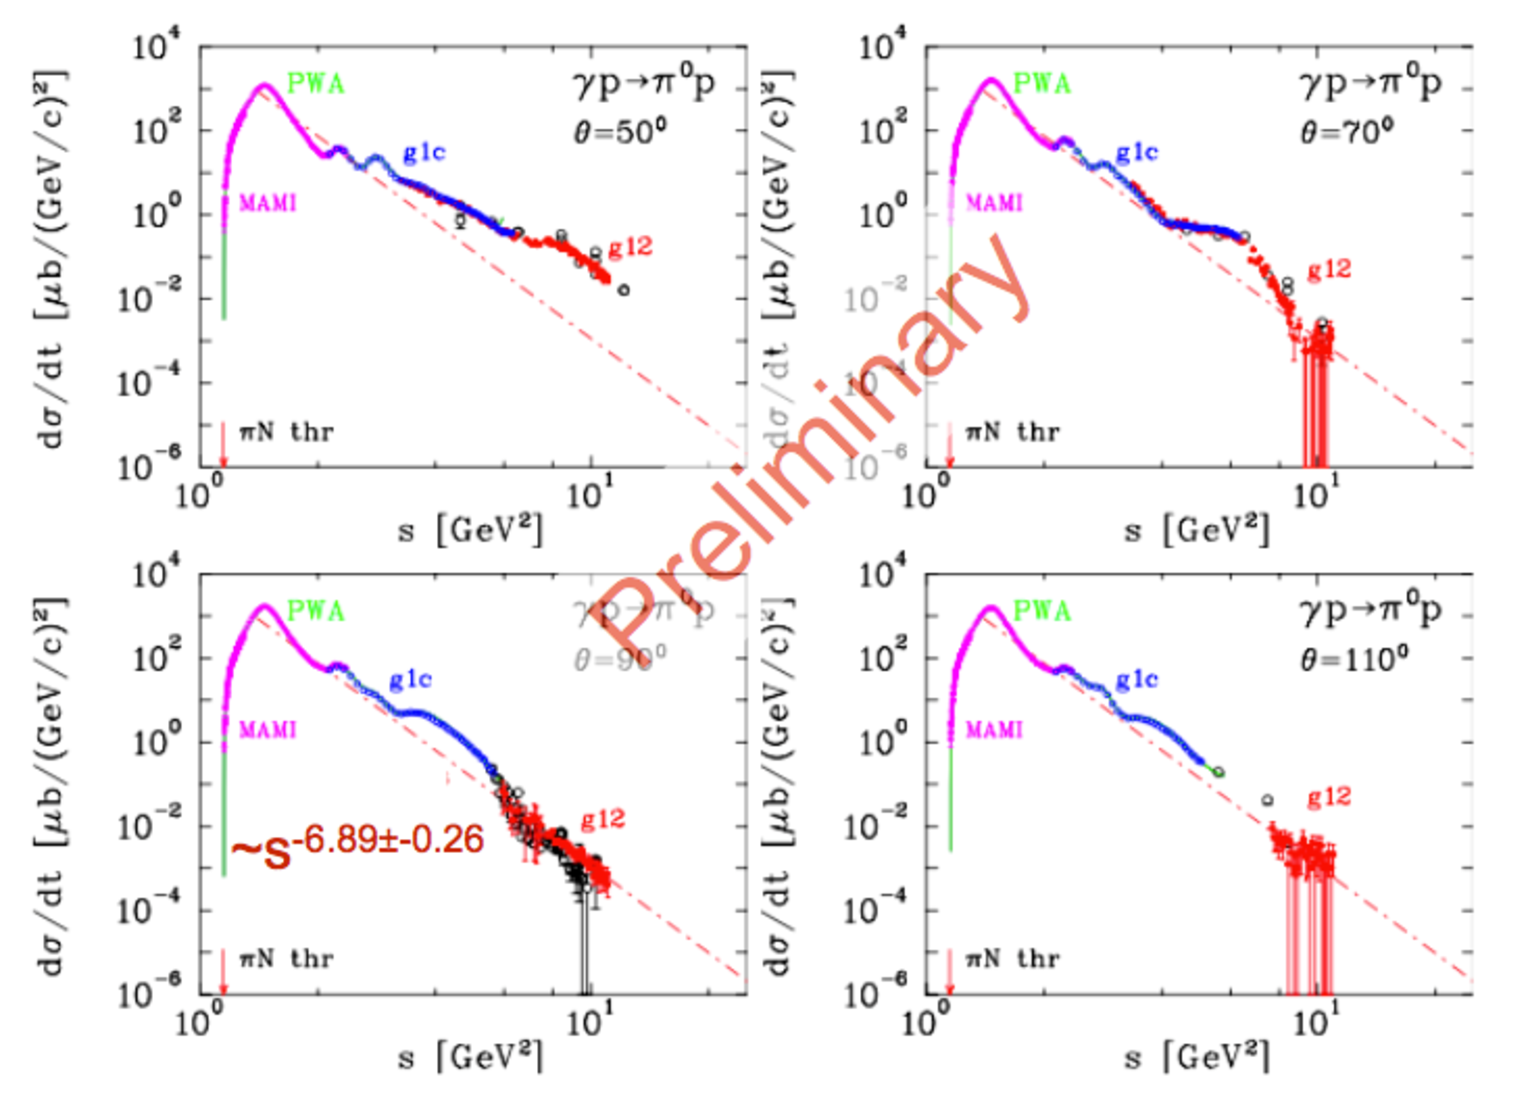
\includegraphics[width=250 pt]{\figures/analysis/DSG/pi0_scaling.pdf}}
	\caption{The differential cross section for the $\gamma p \to p \pi^0$ reaction at $\theta_{c.m.}$ = $50^{\circ}$, $70^{\circ}$, $90^{\circ}$, $110^{\circ}$, as a function of s (center of mass energy squared). Experimental data are from the current measurement (red filled circles), CLAS~\protect\cite{Dugger07,Dugger13} (blue circles), MAMI~\protect\cite{beck} (magenta circles), old measurements~\protect\cite{Joos} (black open circle plus). The dash dotted line is a result of the fit performed at $\theta$ = $90^{\circ}$ with power function $\sim s^{−n}$ leading to n = $6.89 \pm 0.26$.}
	\label{fig:pi0_scaling}
\end{figure}